\documentclass[conference]{IEEEtran}
\usepackage{amsmath}
\usepackage{amssymb}
\usepackage{mathtools}
\usepackage{algorithmic}
\usepackage{subfigure}
\usepackage{tikz}
\newlength\figureheight
\newlength\figurewidth
%\usepackage{url}

% correct bad hyphenation here
\hyphenation{op-tical net-works semi-conduc-tor}

%%%%%%%%%%%%%% COMMANDS
\newcommand{\alg}{RQ-Learning\xspace}

\newcommand{\Rmodel}{\mathcal{R}}
\newcommand{\Pmodel}{\mathcal{P}}
\newcommand{\Rparams}[1][]{\boldsymbol{\omega}^{#1}}
\newcommand{\Rpspace}{\Omega}
\newcommand{\Rbasis}[1][]{\boldsymbol{\phi}\left({#1}\right)}
\newcommand{\Rmodelp}[1][\Rparams]{\mathcal{R}^{#1}}
\newcommand{\Rspace}[1][\dobj-1]{\Delta^{#1}}
\newcommand{\Simplex}[1][\dobj-1]{\mathbb{D}^{#1}}
\newcommand{\Rparamsdom}{\Theta^{*}}

\newcommand{\dsetexp}{\mathcal{D}}
\newcommand{\numdsetexp}{N}

\newcommand{\fe}[2][]{\boldsymbol{\mu}_{#2}\left(#1\right)}  %feature expectation
\newcommand{\feapx}{\widehat{\boldsymbol{\mu}}}                %approximate fe
\newcommand{\jval}[2][]{J_{#2}\left({#1}\right)}
\newcommand{\djval}[2][]{\Delta J_{#2}\left({#1}\right)}
\newcommand{\poly}{\mathcal{P}}
\newcommand{\radius}{r}
\newcommand{\acval}{\rho}
\newcommand{\targetset}{\mathbb{X}^{\epsilon}}

\newcommand{\dpolycut}{m}

\newcommand{\JvalMO}[2][\pi]{\boldsymbol{J}_{#2}\left(#1\right)}
%%%%%%%%%%%%%%%%%%%%%%%



%% math commands
\newcommand{\transpose}[1]{{#1}^\texttt{T}}
\DeclareMathOperator*{\argmax}{arg\,max}
\DeclareMathOperator*{\argmin}{arg\,min}
\DeclareMathOperator*{\EV}{\mathbb{E}}
\DeclareMathOperator*{\var}{\textbf{\texttt{Var}}}
\DeclareMathOperator*{\gradp}{\nabla_{\ppvect}}
\DeclareMathOperator*{\gradhp}{\nabla_{\hpvect}}

\newcommand{\norm}[2][\infty]{\left\|#2\right\|_{#1}}

\newcommand{\realspace}{\mathbb R}		% realspace

\newcommand{\statespace}{\mathcal X}		% state space
\newcommand{\actionspace}{\mathcal U}		% action space
\newcommand{\pmodel}{\mathcal P}		% transition function
\newcommand{\rmodel}{\mathcal R}		% reward function
\newcommand{\initD}{D}				% initial distribution

%% Vector and Matrix
\newcommand{\rvect}{\mathbf{R}}			% reward vector
\newcommand{\vvect}{\mathbf{V}}			% value function vector
\newcommand{\jvect}{\mathbf{J}}			% score vector
\newcommand{\gammavect}{\boldsymbol{\gamma}}	% gamma vector
\newcommand{\pmtx}{\mathbf{P}}			% transition matrix


\newcommand{\ppspace}{\Theta}
\newcommand{\pp}{\theta} 			% policy params
\newcommand{\ppvect}{\boldsymbol{\pp}}		% policy params vector (bold)
\newcommand{\vecop}{\text{vec }}
\newcommand{\sap}{\boldsymbol{z}}

\newcommand{\hpvect}{\boldsymbol \rho}
\newcommand{\hyperdist}{}

\newcommand{\Jvalapx}[1][\ppvect]{\widehat{J}\left({#1}\right)}
\newcommand{\Jval}[1][\ppvect]{J\left({#1}\right)}
\newcommand{\Jvalp}[2][\ppvect]{J_{#2}\left({#1}\right)}
\newcommand{\Mval}[1][\ppvect]{M\left({#1}\right)}
\newcommand{\Jvalvect}[1][\ppvect]{\jvect\left({#1}\right)}
\newcommand{\offJval}[1][\ppvect]{\mathcal{J}\left({#1}\right)}

\newcommand{\dstate}{n}
\newcommand{\daction}{m}
\newcommand{\dobj}{q}
\newcommand{\dpolicy}{d}

\newcommand{\numtraj}{N}

\newcommand{\horiz}{T}
\newcommand{\traj}{\tau}
\newcommand{\trajset}{\mathcal{T}}
\newcommand{\trajspace}{\mathbb{T}}
\newcommand{\trajlength}{T}
\newcommand{\trajR}{R}
\newcommand{\pdfunc}[1]{p\left(#1\right)}

\newcommand{\currstep}{t}	% index for current time step in GPOMDP derivations
\newcommand{\indxlogpi}{i}	% index for \sum \nabla log policy
\newcommand{\indxr}{j}		% index for \sum reward
\newcommand{\indxis}{w}		% index  for \prod importance sampling
\newcommand{\indxint}{k}	% index for \prod \int
\newcommand{\indxcomp}{k}	% index for \theta or gradient components
\newcommand{\indxcompr}{h}	% index for reward or gradient components

\newcommand{\Hessian}{\mathcal{H}}
\newcommand{\HJ}[1][\ppvect]{\Hessian_{\ppvect}\jvect({#1})}
\newcommand{\HJhat}[1][\ppvect]{\widehat{\Hessian}_{\ppvect}\jvect({#1})}
\newcommand{\HJREF}[1][\ppvect]{\widehat{\Hessian}_{\ppvect}^{RF}\jvect({#1})}
\newcommand{\HJGP}[1][\ppvect]{\widehat{\Hessian}_{\ppvect}^{GP}\jvect({#1})}
\newcommand{\glp}[1][]{\nabla_{\ppvect} \log \pi_{\ppvect}(a_{#1}|s_{#1})}
\newcommand{\hlp}[1][]{H_{\ppvect} \log \pi_{\ppvect}(a_{#1}|s_{#1})}

\newcommand{\EVV}[2][\ppvect \in \ppspace]{\EV_{#1}\left[{#2}\right]}
\newcommand{\EVVC}[3]{\EV_{\substack{#1}}\left[{#2}\middle|{#3}\right]}

\newcommand{\cMtx}[1][]{\mathcal{C}\left(#1\right)}
\newcommand{\basegrad}{b_{\nabla}}
\newcommand{\baseline}{b_\indxcomp}
\newcommand{\stepbaseline}{b^{(\currstep)}_\indxcomp}
\newcommand{\baseF}{F^{(\traj)}}
\newcommand{\baseG}{G_\indxcomp^{(\traj)}}
\newcommand{\stepbaseF}{F^{(\currstep)}}
\newcommand{\stepbaseG}{G_\indxcomp^{(\currstep)}}
\newcommand{\varr}[1][]{\textbf{\texttt{Var}}\left( {#1}\right)}

\newcommand{\pol}{\pi}
\newcommand{\polb}{\pi^{\mathcal{B}}}
\newcommand{\polt}{\pi^{\mathcal{T}}}

\newcommand{\qf}[1][^\pol]{Q#1}
\newcommand{\qffun}[2]{Q#1\left(#2\right)}		% value function with parenthesis

\newcommand{\mow}{\boldsymbol{\alpha}}
% \newcommand{\mow}{\Rparams}

\newcommand{\normv}{x}
\newcommand{\normpow}{y}
\newcommand{\ncost}[1][_{\normv}^{\normpow}]{\mathcal{C}{#1}}

\newcommand{\mdp}{\mathcal{M}}

\newcommand{\texsub}[1]{\textsc{\tiny #1}}


\usepackage{xspace}
\DeclareRobustCommand{\eg}{e.g.,\@\xspace}
\DeclareRobustCommand{\ie}{i.e.,\@\xspace}
\DeclareRobustCommand{\wrt}{w.r.t.\@\xspace}

%%
\newtheorem{Property}{Property}
\newtheorem{theorem}{Theorem}

% Q decomposition commands
\newcommand{\Rtilde}{\widetilde{R}}
\newcommand{\Qtilde}{\widetilde{Q}}


\begin{document}

\title{Exploiting Structure and Uncertainty of Bellman Updates in Markov Decision Processes}

% author names and affiliations
% use a multiple column layout for up to three different
% affiliations
\author{\IEEEauthorblockN{Davide Tateo, Carlo D'Eramo, Alessandro Nuara, Marcello Restelli, Andrea Bonarini}
\IEEEauthorblockA{Department of Electronics, Information and Bioengineering\\
Politecnico Di Milano, Milano, Italy\\
Email: \{davide.tateo, carlo.deramo,  alessandro.nuara, marcello.restelli, andrea.bonarini\}@polimi.it}
}

% make the title area
\maketitle

% As a general rule, do not put math, special symbols or citations
% in the abstract
\begin{abstract}
In many real-world problems stochasticity is a critical issue for the learning process. The sources of stochasticity come from the transition model, the explorative component of the policy or, even worse, from noisy observations of the reward function. For a finite number of samples, traditional Reinforcement Learning (RL) methods provide biased estimates of the action-value function leading to poor estimates and propagating them by the application of the Bellman operator. While some approaches rely on the fact that the estimation bias is the key problem in the learning process, we show that in some cases this assumption does not necessarily hold. We propose a method that exploits the structure of the Bellman update and the uncertainty of the estimation in order to better use the amount of information provided by the samples. We show theoretical considerations about this method and its relation w.r.t. Q-Learning. Moreover, we test it in environments available in literature in order to demonstrate its effectiveness against other algorithms that focus on bias and sample-efficiency.
\end{abstract}

% no keywords


% For peer review papers, you can put extra information on the cover
% page as needed:
% \ifCLASSOPTIONpeerreview
% \begin{center} \bfseries EDICS Category: 3-BBND \end{center}
% \fi
%
% For peerreview papers, this IEEEtran command inserts a page break and
% creates the second title. It will be ignored for other modes.
\IEEEpeerreviewmaketitle

\section{Introduction}
It is well known that a key issue of Reinforcement Learning (RL) problems is the accuracy of the estimation of the action-value with a limited number of samples. While most algorithms guarantee the convergence of the estimates to the optimal action-value, in practice the presence of stochastic components lead to slow learning. In fact, the majority of real-world problems have significant sources of stochasticity: the environment could have stochastic transition and this complicates the estimation of the effectiveness of an action; most of the times it is necessary to use stochastic policies to guarantee that all states are visited infinitely many times, that is required to guarantee the convergence of the algorithm; the policy could change during the learning process resulting in very different behaviors; the reward function is often corrupted by noisy observations and, in other cases, the reward function is stochastic itself. Moreover, it usually happens that some deterministic environments are partially observable and, thus, are perceived by the agent as stochastic decision processes (e.g. Blackjack).

Since Monte-Carlo estimates of action-values are affected by high variance of the returns, the most successful RL algorithms are based on bootstrapping (e.g. Q-Learning \cite{watkins1992q}), that trades off the variance of the estimation with a consistent but biased estimator. However, with a finite number of samples, the bias of the estimation could be significantly relevant when propagating the action-values to the next state and, recursively, to all the other states. Recent works tried to deal with this issue, in particular focusing on the estimation of the maximum expected value. 
It is well known \cite{smith2006optimizer, van2004rational} that the maximum operator (used in the Q-Learning update equation) is positively biased, thus it overestimates the optimal action-value. In highly stochastic environments, this overestimation leads to unstable learning and poor convergence rates. In order to avoid this issue, the Double Q-Learning algorithm \cite{van2010double} has been proposed. This algorithm uses the double estimator \cite{van2013estimating} to compute the maximum action-value to calculate the temporal-difference error: providing a negatively biased estimation (i.e. underestimating) of the maximum action-value, this approach can improve the performance especially in noisy environments.
Another recently proposed approach is the Weighted Q-Learning \cite{d2016estimating} that computes a weighted average of the action-value functions estimates balancing between underestimation and overestimation.

However, an inaccurate estimation of the action value function does not always imply bad performance; indeed most of the policies are not dependent on the accuracy of the action-values, but instead they rely on their ordering. For instance, in the empirical section of this paper, we show how Speedy Q-Learning algorithm \cite{NIPS2011_4251} reaches very good performance despite sometimes estimating the action-values very poorly. Starting from this considerations, we try to address this problem from another point of view. Indeed, we do not focus on the estimation of the maximum expected value, but we care about weighting the new samples according to the uncertainty of the current estimates.
In fact, we propose this work starting from the consideration that it is not sufficient to accurately estimate the maximum expected value of the Q-function of the next state, but we also need to consider how these information are propagated to other states.

The interesting aspect of this approach is that it is possible to use any maximum expected value estimator and, moreover, it can be easily extended in an on-policy scenario. Since we believe that the choice of the estimator is not a relevant issue in our approach, we choose the maximum operator as it is the simplest one.

\section{Preliminaries}
---TODO preso dal mio paper, va parafrasato, solo modifiche minori--
A Markov Decision Process (MDP) is defined by $\mathcal{M} = \langle \statespace,\actionspace,\Pmodel,\gamma,\Rmodel, D\rangle$, where $\statespace$ is the state space, $\actionspace$ is the action space, $\Pmodel$ is a Markovian transition model where $\Pmodel(x'|x,u)$ defines the transition density between state $x$ and $x'$ under action $u$, $\gamma\in[0,1)$ is the discount factor, $\Rmodel(r|x, u, x')$ defines the distribution of the reward, and $D$ is the distribution of the initial state.
A stochastic policy is defined by a density distribution $\pol(\cdot|x)$ that specifies for each state $x$ the density distribution over the action space $\actionspace$.
---
Given a policy $\pol$, we define the action value function as:
\begin{align}
 Q^\pol(x,u)=\underset{\strut\mathclap{\substack{(x', u')\sim \\ \Pmodel(x'|x,u)\pol(u'|x')}}}{\mathbb{E}}\left[ r(x,u,x')+\gamma Q^\pol(x,u)(x',u')\right].
 \label{eq:qpol}
\end{align}

The optimal policy $\pol*$ is the policy with the highest expected return in the MDP. The optimal action-value function $Q^*(x, u)$ is the action-value function of the optimal policy.
It has been shown that the optimal policy in any MDP can be always a deterministic policy that at each state chooses the action with the highest $Q^*(x, u)$ value.
Given that we can always write the optimal action-value function as:
\begin{align}
 Q^*(x,u)=\underset{\strut\mathclap{x'\sim \Pmodel(x'|x,u)}}{\mathbb{E}}\left[ r(x,u,x')+\gamma\max_{u'} Q^*(x',u')\right].
 \label{eq:qopt}
\end{align}
As the expected value is a linear operator, we can always write (\ref{eq:qopt}) as:
\begin{align}
 Q^*(x,u)=\underset{\strut\mathclap{x'\sim \Pmodel(x'|x,u)}}{\mathbb{E}}\left[ r(x,u,x')\right]+\underset{\strut\mathclap{x'\sim \Pmodel(x'|x,u)}}{\gamma\mathbb{E}}\left[ \max_{u'} Q^*(x',u')\right].
 \label{eq:qdec}
\end{align}

We now introduce two functions, $\Rtilde$ and $\Qtilde$, defined as:
\begin{align}
 \Rtilde(x,u)&=\underset{\strut\mathclap{x'\sim \Pmodel(x'|x,u)}}{\mathbb{E}}\left[ r(x,u,x')\right], \nonumber\ \\
 \Qtilde(x,u)&=\underset{\strut\mathclap{x'\sim \Pmodel(x'|x,u)}}{\mathbb{E}}\left[\max_{u'} Q^*(x',u')\right].
 \label{eq:rqtilde}
\end{align}
We can give an interpretation of these two functions. $\Rtilde(x,u)$ is the expected immediate reward of the action $u$ in the state $x$. $\Qtilde(x,u)$ is the expected discounted return of the states reached after performing action $u$ in state $x$, i.e. the expected gain of the reached state.

We can now write the optimal value function as:
\begin{align}
 Q^*(x,u)=\Rtilde(x,u)+\gamma\Qtilde(x,u).
 \label{eq:qdecrqtilde}
\end{align}

Our approach shifts the focus of the RL task from finding a good estimator for the optimal action-value function, to the task of finding good estimators for the $\Rtilde$ and $\Qtilde$ functions. The main motivation is that the sources of uncertainty of the two components of the action-value function are different: the $\Rtilde$ function only depends on the transition and reward models, while $\Qtilde$ also depends on the optimal policy.

\section{The Proposed Method}

In the following section we derive our method from (\ref{eq:qdecrqtilde}). We propose the general schema, using the maximum estimator and we show the relations with the standard Q learning update. We call this method \emph{\alg} as it decomposes the TD-Error in a reward component and an action-value component.

\subsection{Decomposition of the TD Error}

Standard Q-Learning algorithm computes the temporal difference error given the tuple $(x,u,r,x')$ w.r.t. the current action-value estimates, and then updates such estimate proportionally to the error. The amount of correction in the direction of the new sample is measured by the learning rate: if the learning rate equals to $1$, the new sample substitutes the old estimate; if the learning rate equals to $0$, the new sample is discarded, and the old estimate is kept unchanged. 
As shown in (\ref{eq:qdecrqtilde}) the action-value function could be decomposed in two different components. Our method is based on the idea to give separate estimates for these two components, instead of computing a TD error, we compute the error w.r.t. each component of the action-value function:

\begin{align}
\Rtilde_{t+1}(x,u) & \leftarrow\Rtilde_t(x,u)+\alpha_t(R(x,u,x')-\Rtilde_t(x,u)), \label{eq:rtilupdedate}\\
\Qtilde_{t+1}(x,u) & \leftarrow\Qtilde_t(x,u)+\beta_t(\max_{u'}Q_t(x',u')-\Qtilde_t(x,u)).
\label{eq:qtildeupdate}
\end{align}
Separating the two components of the value function can be useful, as the two components have inherently different sources of stochasticity. Moreover, the information stored in $\Rtilde$ is local to each state-action pair, and does not contain the uncertainty of the estimation of others states. The information stored in $\Qtilde$ instead depends only on the action-value function of the states that could be reached after performing the action $u$ in the state $x$, which depends, recursively, on the other action-value functions. It is clear that the propagation of uncertain values only affects the $\Qtilde$ component.
As the actual action value function is the sum of the two estimates, we can write an equivalent update for the Q function:

\begin{align}
Q_{t+1}(x,u)\leftarrow&\Rtilde_t(x,u)+\alpha_t(R(x,u,x')-\Rtilde_t(x,u)) \nonumber\\
  & +\gamma\left(\Qtilde_t(x,u)+\beta_t(\max_{u'}Q_t(x',u')-\Qtilde_t(x,u))\right) \nonumber\\
= & Q_t(x,u)+\alpha_t(R(x,u,x')-\Rtilde_t(x,u)) \nonumber\\
  & +\gamma\beta_t(\max_{u'}Q_t(x',u')-\Qtilde_t(x,u))
 \label{eq:cumulativeupdate}
\end{align}
notice that this update cannot be used in practice in the algorithm, as it is not keeping the current values of the single components. However (\ref{eq:cumulativeupdate}) is useful to analyze the relations to standard Q-Learning algorithm.

\subsection{Analysis of the Decomposed Update}
We will discuss the relationship of our method with standard temporal difference methods. Let $t$ be the learning step. As a first step of our analysis we can consider the simplest case $\alpha_t=\beta_t$, $\forall t$ by combining (\ref{eq:cumulativeupdate}) and (\ref{eq:qdecrqtilde}) we obtain:
\begin{align}
Q_{t+1}(x,u) \leftarrow & Q_t(x,u)+\alpha_t(R(x,u,x')+\gamma\max_{u'}Q_t(x',u')\nonumber\\
 & - Q_t(x,u))
\end{align}
That is the classical Q-Learning update. 

We consider now the setting $\alpha_t\geq\beta_t>0$, $\forall t$. Let $\beta_t=\delta_t\alpha_t$, we obtain:
\begin{align}
Q_{t+1}(x,u) \leftarrow & Q_t(x,u)+\alpha_t(R(x,u,x')+\gamma\delta_t \max_{u'}Q_t(x',u') \nonumber\\
  & -(\Rtilde_t(x,u)+\gamma\delta_t\Qtilde_t(x,u))) \nonumber\\
= & Q_t(x,u)+\alpha_t(R(x,u,x')+\gamma_t'\max_{u'}Q_t(x',u') \nonumber\\
  & -(\Rtilde_t(x,u)+\gamma_t'\Qtilde_t(x,u))) \nonumber\\
= & Q_t(x,u)+\alpha_t((R(x,u,x')+\gamma_t'\max_{u'}Q_t(x',u')) \nonumber\\
  & - Q_t'(x,u))
\end{align}
with $\gamma_t'=\gamma\delta_t$. Notice that $Q_t'(x,u)$ is the current Q function, but computed with a different discount factor. If the condition above is satisfied, then we can see our method as a variable discount factor learning. If we consider $\delta_t$ that increases monotonically in the interval $[0,1]$, our method works increasing the effective horizon each step, starting from trying to solve a greedy myopic problem and moving towards the real one. This approach has been used in practice to solve infinite horizon problems when the discount factor is close to $1$ ~\cite{crites1996improving, bao2008infinite, franccois2015discount}.

Finally, we can observe that if the reward function and the transition model are deterministic, we can use $\alpha=1$ and consider only $\beta_t=\delta_t$.

\subsection{Variance dependent learning rate}
To improve performance on the estimation, we would like to weight the error of each sample w.r.t. the current estimate depending on how much we are sure about the current value of our estimate. Thus, we propose a learning rate that depends on the variance of the current variable estimate.

First of all we need to compute the variance of each estimator. To perform such computation we have to make the assumption that the learning rates are independent from the data. Of course, we violate this assumption, but it is needed in order to have a closed form for the variance of the estimator and works well in practice. We will suppose also that the samples $X_i$ are i.i.d., with mean $\mu$ and variance $\sigma^2$. Consider the general form of the estimator:

\begin{align}
 \widetilde{X}_{n+1} = (1-\alpha_t)\widetilde{X}_{n}+\alpha_tX_{n}
\end{align}
We now compute the expected value and the variance of this estimator:
\begin{align}
 \mathbb{E}\left[\widetilde{X}_{n+1}\right]& = \mu\sum_i^n \alpha_i \prod_{j=i+1}^{n} \left(1-\alpha_j\right)\\
 \mathrm{Var}\left[\widetilde{X}_{n+1}\right]& = \sigma^2\sum_i^n \alpha_i^2 \prod_{j=i+1}^{n} \left(1-\alpha_j\right)^2 = \sigma^2\omega
\end{align}
with $\omega=\sum_i^n \alpha_i^2 \prod_{j=i+1}^{n} \left(1-\alpha_j\right)^2$. Notice also that we can use the sample covariance $S_{n-1}$ of the random variable $X$ to estimate the real covariance $\sigma^2$. It is possible to compute in an incremental way both the sample covariance, in the traditional way, and $\omega$:

\begin{align}
 \omega_{n+1}=(1-\alpha_n)^2\omega_n+\alpha_n^2
\end{align}
A weak assumption of this model is that the variables are identically distributed. While this should be true for the reward function, if the MDP is stationary, this is not true for the Q function values whose distribution is affected by the policy and by the other states current estimates. However, a good approximation, could be to consider data collected in a temporal window in which the distribution is approximately stationary: using such approach, we can compute the variance of the process in a given time window forgetting old values that can lead to a biased estimation of the current window variance. While this approach is not formally correct, as the derivation of the variance estimates makes the assumption of i.i.d. variables, this approximation leads to very good results in practice as we show in the empirical Section \ref{S:empirical}.

Finally, we can choose a learning rate that depends on the covariance. Let $\sigma_e^2(t)$ be an estimate of $\mathrm{Var}\left[\widetilde{X}_{t}\right]$. We propose the following learning rate for each component of the action-value function:

\begin{align}\label{eq:alpha_eq}
 \alpha_t=\dfrac{\sigma_e^2(t)}{\sigma_e^2(t)+\eta}
\end{align}
where $\eta$ is the amount of the estimator variance for which the learning rate is $0.5$ (i.e. when $\sigma_e=\eta$ the learning rate is 0.5). It can be seen as a soft threshold to tune the speed of the decrease of the learning rate w.r.t. the estimator variance.

If we consider the case $\beta_t=\alpha_t\delta_t$, then we have to use a different learning rate. As we want an increase of the discount factor faster than the decrease of the general learning rate, we can use an exponentially increasing learning rate for the delta parameter:

\begin{align}\label{eq:delta_eq}
 \delta(t) = e^{\frac{\sigma_e^2}{\eta}\log(0.5)}
\end{align}

Where $\eta$ has the same interpretation of the previous scenario.

\subsection{Discussion on convergence}

Althought we do not have strong results about convergence of this method if using the variance dependent learning rate, we designed the variance dependent learning rate functions with the convergence in mind.

Suppose that the variance of the estimator $\sigma_e^2(t)$ is a variance of the sample mean. Is well known, by the central limit theorem, that the variance of the sample mean is $\sigma_{\mu}(t)=\dfrac{\sigma^2}{t}$, where $\sigma$ is the variance of the process that generate samples.
This assumption is in general false, as we can see from the formula of the learning rate, however in some cases this could be a good approximation,as the sample mean is a special case of the estimator.

Now, just consider the proposed learning rate in (\ref{eq:alpha_eq}), substituting the sample mean into the variance of the estimator:

\begin{align}\label{eq:alpha_smv}
 \alpha_t=\dfrac{\sigma^2}{\sigma^2+\eta t}
\end{align}

It can be easily shown that:
\begin{align}
 \lim_{N\rightarrow\infty} \sum_{t=0}^{N}\dfrac{\sigma^2}{\sigma^2+\eta t} & \rightarrow\infty \\
 \lim_{N\rightarrow\infty} \sum_{t=0}^{N}\left(\dfrac{\sigma^2}{\sigma^2+\eta t}\right)^2 & =K
\end{align}

Now, consider $\beta_t=\alpha_t\delta_t$. In this scenario we proposed an exponential learning rate. Let $\alpha_t=\dfrac{1}{t}$ for simplicity.
now consider the learning rate (\ref{eq:delta_eq}), substituting the sample mean into the variance of the estimator:

\begin{align}\label{eq:beta_delta_smv}
 \beta(t) = \dfrac{1}{t}e^{\frac{\sigma^2}{\eta t}\log(0.5)}
\end{align}


It can be easily shown that:
\begin{align}
 \lim_{N\rightarrow\infty} \sum_{t=0}^{N}\dfrac{1}{t}e^{\frac{\sigma^2}{\eta t}\log(0.5)} & \rightarrow\infty \\
 \lim_{N\rightarrow\infty} \sum_{t=0}^{N}\left(\dfrac{1}{t}e^{\frac{\sigma^2}{\eta t}\log(0.5)}\right)^2 & =K
\end{align}

Unfortunately, the analysis of the generic variance estimator is more complex. We suppose that convergence could be assured with some mild conditions on $\eta$ and $\sigma$.


\section{Experimental Results}\label{S:empirical}
In this section, we highlight the main advantages of exploiting the structure of the TD-Error with \alg in three discrete MDPs. We compare \alg against Q-Learning \cite{watkins1992q}, Double Q-Learning \cite{van2010double}, Weighted Q-Learning \cite{d2016estimating} and Speedy Q-Learning\footnote{In these experiments we consider the asynchronous version of Speedy Q-Learning.} \cite{NIPS2011_4251}. We choose this set of algorithms because we want to analyze the impact of the maximum expected value estimator in the learning process. Indeed, while \cite{van2010double} strongly suggests that a negatively biased estimator should be used to deal with stochastic MDPs, the following empirical results will show that positively biased estimators are able to achieve better performance in highly stochastic problems as well. We want to show that instead the main point consists in exploiting data in the best way, in particular in the estimation of the action-value, giving higher relevancy to more recent samples. We conjecture that the trade-off between keeping the old estimate and updating it with the new one is the key issue in highly stochastic environments. Both \alg and Speedy Q-Learning exploit this idea, in particular the latter uses an increasing learning rate on the difference between the target computed with the current estimation and the one computed with the previous estimation; on the other hand \alg weights the update considering the uncertainty of the current estimation.

We analyze the performance of \alg with different choices of learning rates. All the other algorithms use a decaying learning rate $\alpha(s, a) = \frac{1}{n(s, a)^{k}}$ where $n(s, a)$ and $k$ are respectively the number of updates for each action $a$ in state $s$ and a coefficient to tune the rate of decay.\footnote{Assuming that Double Q-Learning splits the action-value table in a table A and a table B, also the learning rate are split in $\alpha_A(s, a) = \frac{1}{n_A(s, a)^{k}}$ and $\alpha_B(s, a) = \frac{1}{n_B(s, a)^{k}}$ where $n_A(s, a)$ and $n_B(s, a)$ are the number of updates for each action $a$ in state $s$, respectively in table A and table B.}

\begin{figure}[t]
\begin{minipage}{\columnwidth}
\centering
  \subfigure[$\alpha = \dfrac{1}{n(s,a)}$\label{F:hasselt_all_1}]{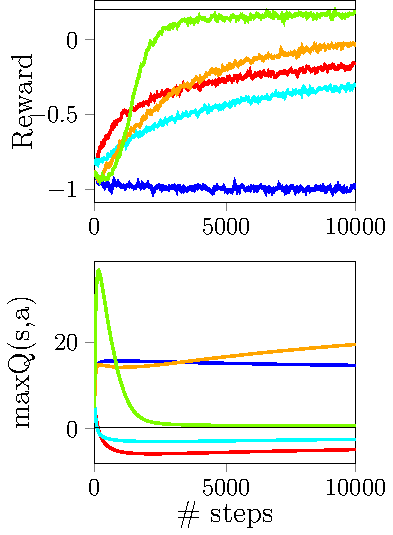
\includegraphics[scale=.7]{./imgs/gridHasselt/allAlgs1.pdf}}\hspace{-.5cm}
  \subfigure[$\alpha = \dfrac{1}{n(s,a)^{0.8}}$\label{F:hasselt_all_08}]{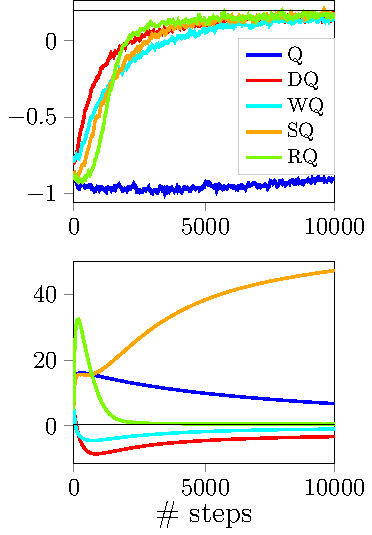
\includegraphics[scale=.7]{./imgs/gridHasselt/allAlgs08.pdf}}
\end{minipage}
  \caption{Mean reward per step (top) and maximum action-value estimate in the initial state (bottom) of all the other algorithms and of the best setting of \alg for this experiment. Results are averaged over $10000$ experiments.}
  \label{F:hasselt_all}
\end{figure}
\begin{figure}[t]
\begin{minipage}{\columnwidth}
\centering
  \subfigure[$\alpha = \dfrac{1}{n(s,a)}$\label{F:hasselt_qdec_1}]{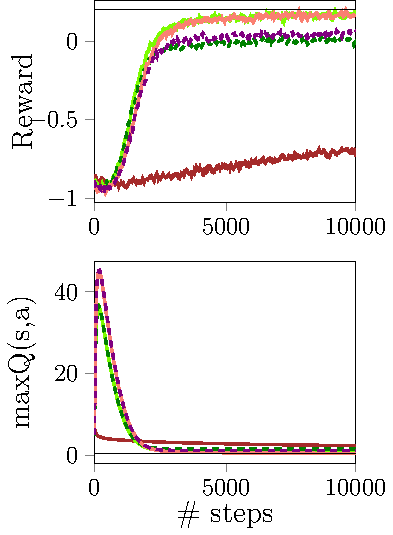
\includegraphics[scale=.7]{./imgs/gridHasselt/QDecs1.pdf}}\hspace{-.5cm}
  \subfigure[$\alpha = \dfrac{1}{n(s,a)^{0.8}}$\label{F:hasselt_qdec_08}]{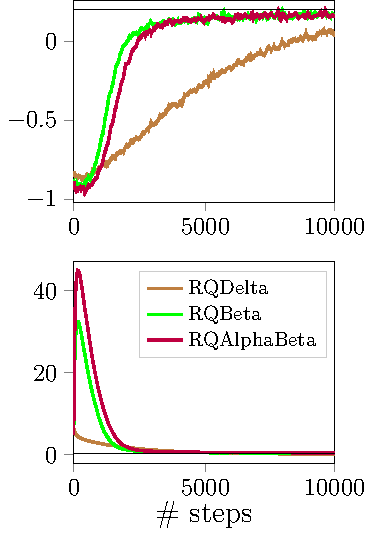
\includegraphics[scale=.7]{./imgs/gridHasselt/QDecs08.pdf}}
\end{minipage}
  \caption{Mean reward per step (top) and maximum action-value estimate in the initial state (bottom) of the best setting of \alg for this experiment together with other less effective setting of \alg. Results are averaged over $10000$ experiments.}
  \label{F:hasselt_QDecs}
\end{figure}

\begin{figure*}[t]
\begin{minipage}{\textwidth}
\centering
  \subfigure[$\alpha = \dfrac{1}{n(s,a)}$\label{F:double_chain_1_1}]{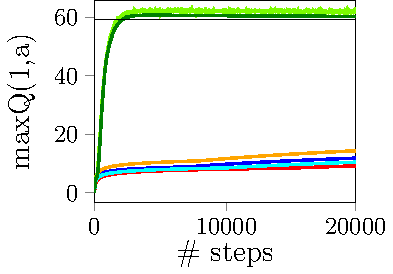
\includegraphics[scale=.7]{./imgs/doubleChain/v1-1.pdf}}
  \subfigure[$\alpha = \dfrac{1}{n(s,a)^{0.51}}$\label{F:double_chain_1_51}]{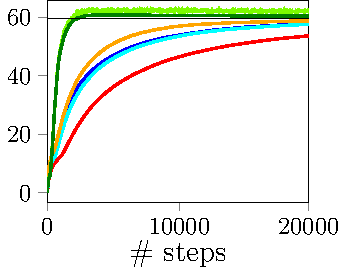
\includegraphics[scale=.7]{./imgs/doubleChain/v1-51.pdf}}
  \subfigure[$\alpha = \dfrac{1}{n(s,a)}$\label{F:double_chain_5_1}]{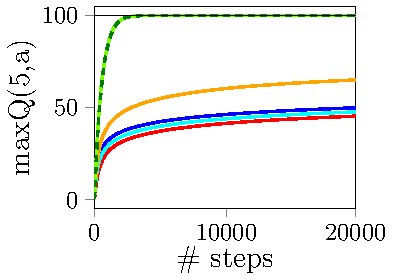
\includegraphics[scale=.7]{./imgs/doubleChain/v5-1.pdf}}
  \subfigure[$\alpha = \dfrac{1}{n(s,a)^{0.51}}$\label{F:double_chain_5_51}]{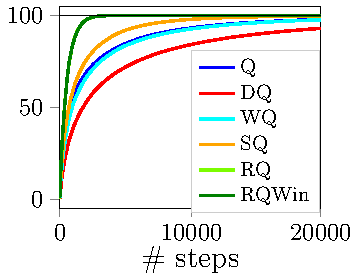
\includegraphics[scale=.7]{./imgs/doubleChain/v5-51.pdf}}
\end{minipage}
\caption{Maximum action-value estimate in state $1$ (\ref{F:double_chain_1_1}, \ref{F:double_chain_1_51}) and state $5$ (\ref{F:double_chain_5_1}, \ref{F:double_chain_5_51}). Results are averaged over $500$ experiments.}
  \label{F:double_chain_q}
\end{figure*}

\begin{figure*}[t]
\begin{minipage}{\textwidth}
\centering
  \subfigure[$\alpha = \dfrac{1}{n(s,a)}$\label{F:lrs_1_1}]{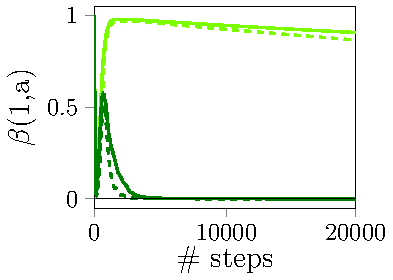
\includegraphics[scale=.7]{./imgs/doubleChain/lrs1-1.pdf}}
  \subfigure[$\alpha = \dfrac{1}{n(s,a)^{0.51}}$\label{F:lrs_1_51}]{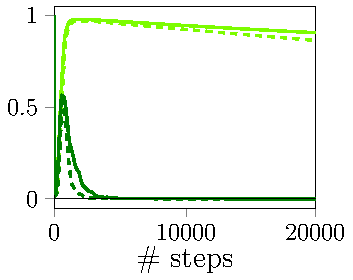
\includegraphics[scale=.7]{./imgs/doubleChain/lrs1-51.pdf}}
  \subfigure[$\alpha = \dfrac{1}{n(s,a)}$\label{F:lrs_5_1}]{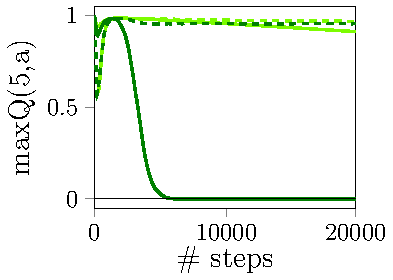
\includegraphics[scale=.7]{./imgs/doubleChain/lrs5-1.pdf}}
  \subfigure[$\alpha = \dfrac{1}{n(s,a)^{0.51}}$\label{F:lrs_5_51}]{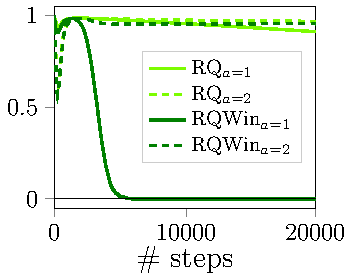
\includegraphics[scale=.7]{./imgs/doubleChain/lrs5-51.pdf}}
\end{minipage}
\caption{Learning rate of the two actions in state $1$ (\ref{F:lrs_1_1}, \ref{F:lrs_1_51}) and state $5$ (\ref{F:lrs_5_1}, \ref{F:lrs_5_51}) for RQ-Learning with and without windowed variance estimation. Results are averaged over $500$ experiments.}
  \label{F:double_chain_lr}
\end{figure*}

\begin{figure*}[t]
\begin{minipage}{\textwidth}
\centering
  \subfigure[$\alpha = \dfrac{1}{n(s,a)}$\label{F:max_a_1}]{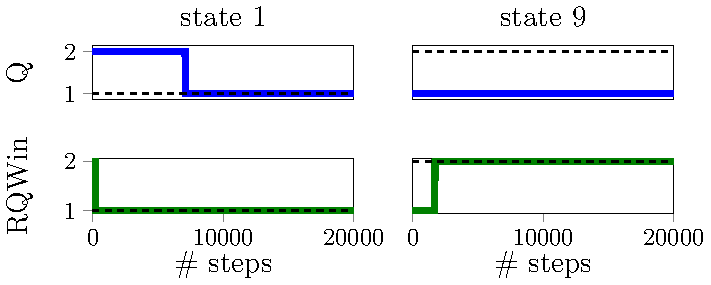
\includegraphics[scale=.7]{./imgs/doubleChain/max_a-1.pdf}}
  \subfigure[$\alpha = \dfrac{1}{n(s,a)^{0.51}}$\label{F:max_a_51}]{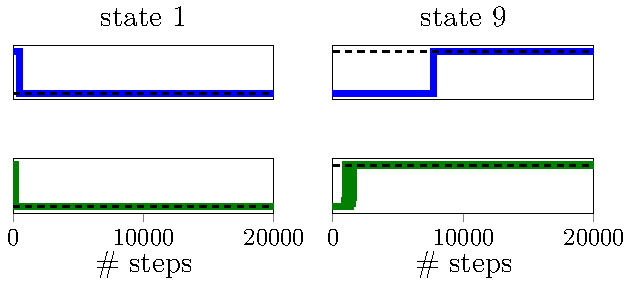
\includegraphics[scale=.7]{./imgs/doubleChain/max_a-51.pdf}}
\end{minipage}
\caption{Action with maximum value in state $1$ and state $9$ for Q-Learning and windowed RQ-Learning.}
  \label{F:max_a}
\end{figure*}

\begin{figure}[t]
\begin{center}
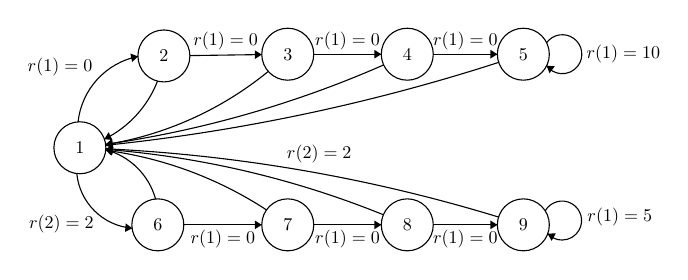
\begin{tikzpicture}[scale=0.11]
\tikzstyle{every node}+=[inner sep=0pt, style={scale=0.65}]
\draw [black] (10.4,-17.1) circle (3);
\draw (10.4,-17.1) node {$1$};
\draw [black] (20.1,-6.5) circle (3);
\draw (20.1,-6.5) node {$2$};
\draw [black] (34.4,-6.3) circle (3);
\draw (34.4,-6.3) node {$3$};
\draw [black] (48.2,-6.3) circle (3);
\draw (48.2,-6.3) node {$4$};
\draw [black] (61.6,-6.3) circle (3);
\draw (61.6,-6.3) node {$5$};
\draw [black] (19.4,-26) circle (3);
\draw (19.4,-26) node {$6$};
\draw [black] (34.4,-26) circle (3);
\draw (34.4,-26) node {$7$};
\draw [black] (48.2,-26) circle (3);
\draw (48.2,-26) node {$8$};
\draw [black] (61.6,-26) circle (3);
\draw (61.6,-26) node {$9$};
\draw [black] (10.195,-14.122) arc (-186.01298:-258.90993:8.628);
\fill [black] (17.12,-6.56) -- (16.23,-6.22) -- (16.43,-7.2);
\draw (11.87,-7.74) node [left] {$r(1)=0$};
\draw [black] (16.449,-26.391) arc (-94.70547:-174.65436:7.013);
\fill [black] (16.45,-26.39) -- (15.69,-25.83) -- (15.61,-26.82);
\draw (8.26,-24.87) node [below] {$r(2)=2$};
\draw [black] (13.375,-17.324) arc (75.15536:15.48481:8.153);
\fill [black] (13.37,-17.32) -- (14.02,-18.01) -- (14.28,-17.05);
\draw [black] (19.363,-9.401) arc (-21.12574:-63.79717:12.497);
\fill [black] (13.22,-16.11) -- (14.16,-16.2) -- (13.72,-15.31);
\draw [black] (32.152,-8.285) arc (-50.72552:-80.81899:39.653);
\fill [black] (13.38,-16.73) -- (14.25,-17.1) -- (14.09,-16.11);
\draw [black] (45.468,-7.539) arc (-66.30261:-81.8066:123.727);
\fill [black] (13.37,-16.71) -- (14.24,-17.09) -- (14.09,-16.1);
\draw [black] (58.752,-7.242) arc (-72.09117:-84.0864:221.864);
\fill [black] (13.39,-16.81) -- (14.23,-17.23) -- (14.13,-16.23);
\draw [black] (13.385,-17.393) arc (82.46666:56.84042:44.631);
\fill [black] (13.39,-17.39) -- (14.11,-17.99) -- (14.24,-17);
\draw [black] (13.394,-17.292) arc (85.54014:67.96192:107.716);
\fill [black] (13.39,-17.29) -- (14.15,-17.85) -- (14.23,-16.86);
\draw [black] (13.398,-17.219) arc (87.26949:73.00835:185.371);
\fill [black] (13.4,-17.22) -- (14.17,-17.76) -- (14.22,-16.76);
\draw (38.03,-18.9) node [above] {$r(2)=2$};
\draw [black] (22.4,-26) -- (31.4,-26);
\fill [black] (31.4,-26) -- (30.6,-25.5) -- (30.6,-26.5);
\draw (26.9,-26.5) node [below] {$r(1)=0$};
\draw [black] (37.4,-26) -- (45.2,-26);
\fill [black] (45.2,-26) -- (44.4,-25.5) -- (44.4,-26.5);
\draw (41.3,-26.5) node [below] {$r(1)=0$};
\draw [black] (51.2,-26) -- (58.6,-26);
\fill [black] (58.6,-26) -- (57.8,-25.5) -- (57.8,-26.5);
\draw (54.9,-26.5) node [below] {$r(1)=0$};
\draw [black] (51.2,-6.3) -- (58.6,-6.3);
\fill [black] (58.6,-6.3) -- (57.8,-5.8) -- (57.8,-6.8);
\draw (54.9,-5.8) node [above] {$r(1)=0$};
\draw [black] (37.4,-6.3) -- (45.2,-6.3);
\fill [black] (45.2,-6.3) -- (44.4,-5.8) -- (44.4,-6.8);
\draw (41.3,-5.8) node [above] {$r(1)=0$};
\draw [black] (23.1,-6.46) -- (31.4,-6.34);
\fill [black] (31.4,-6.34) -- (30.59,-5.85) -- (30.61,-6.85);
\draw (27.23,-5.85) node [above] {$r(1)=0$};
\draw [black] (64.28,-4.977) arc (144:-144:2.25);
\draw (68.85,-6.3) node [right] {$r(1)=10$};
\fill [black] (64.28,-7.62) -- (64.63,-8.5) -- (65.22,-7.69);
\draw [black] (64.117,-24.39) arc (150.34019:-137.65981:2.25);
\draw (68.96,-25.15) node [right] {$r(1)=5$};
\fill [black] (64.41,-27.02) -- (64.86,-27.85) -- (65.35,-26.98);
\end{tikzpicture}
\end{center}
\caption{Structure of the double-chain problem.}
\label{F:double-chain}
\end{figure}

\subsection{Noisy Grid World}
This environment is proposed in \cite{van2010double} and consists in a $3 \times 3$ grid with the initial position in the lower-left cell and the goal state in the upper-right cell. Each action performed in a non-goal state obtains a reward $-12$ and $10$ with equal probability. In the goal state, every action obtains a reward of $5$ and terminates the episode. The discount factor is $\gamma = 0.95$. The policy is $\varepsilon$-greedy with $\varepsilon = \frac{1}{\sqrt{n(s)}}$, where $n(s)$ is the number of  visits of the state $s$. The optimal average reward per step is $0.2$ and the maximum action-value function of the initial state is $5\gamma^4 - \sum_{k=0}^3 \gamma^k \approx 0.36$.

Figure \ref{F:hasselt_all} shows the mean reward per step and the approximation of the maximum action-value in the initial state computed by the other algorithms and \alg with $\alpha$ as used by the other algorithms, but with the separated variance-dependent learning rate $\beta$ for the action-value estimate using $\eta = 1$, that is the most effective setting of \alg that we tried for this problem. Note how the performance of \alg w.r.t. reward are the best one (except for $k=0.8$ where all algorithms perform similarly) and, moreover, how the estimate of the action-value is also the best one. Notice that, with $k=1$, Speedy Q-Learning outperforms both Double Q-Learning and Weighted Q-Learning w.r.t. the mean reward per step, even with a diverging estimate of the action-value function. This is an empirical evidence of our conjecture on the non-correlation of the bias of the estimation, obtained in the experiment proposed in \cite{van2010double} and \cite{d2016estimating}. Moreover, as expected, the performance of \alg is not affected to the exponent used in the learning rate. The other algorithms achieve the optimal performance only in the setting with the higher learning rate, confirming the advantage of giving more importance to newer samples.

In Figure \ref{F:hasselt_QDecs} we compare different variants of \alg: ``RQBeta'' is the same configuration used in Figure \ref{F:hasselt_all}; ``RQDelta'' uses $\beta = \alpha \delta$ with $\eta = 1$; ``RQWin'' uses a windowed estimation of variance with a window of length $50$ and $\eta = 0.5$. ``RQAlphaBeta'' uses a variance-dependent learning rate also for $\alpha$ with $\eta = 100$ and $\beta$ with $\eta = 1$; ``RQWinAlpha'' is the same configuration of the previous one, but uses a windowed $\beta$ with $\eta = 0.5$. Note that $\eta$ has a larger value in configurations without windowed variance estimation because such configurations are likely to overestimate the current variance of the process. ``RQDelta'' configurations result in a cautious learning that leads to very slow improvements, but avoids the overestimation of the action-value slowly converging to the optimal value. While ``RQDelta'' performance are not comparable with other configurations of \alg, it still outperforms Q-Learning. The other configurations perform similarly to the best one.

\subsection{Double Chain}
This is a problem proposed in \cite{Peters2010RelativeEP} which consists in a Markov chain with two branches (Figure \ref{F:double-chain}). In state $1$, action $1$ yields a reward of $0$ and moves the agent in state $2$; action $2$ yields a reward of $2$ and moves the agent in state $6$. In all other states, action $2$ moves the agent in state $1$ and returns a reward of $2$; action $1$ moves the agent in the next state of the chain returning a reward of $0$. In state $5$ and $9$, action $1$ yields a reward of respectively $10$ and $5$. In all states, each action has a probability of success of $0.8$ and, if the action fails, the agent remains in the current state and yields a reward of $0$. The discount factor is $\gamma = 0.9$. The optimal policy is to take action $1$ in state from $1$ to $5$ and action $2$ in the other states. \alg uses $\eta = 10$. In this experiment we focus on the estimation of the action-value function, therefore we use a fully random policy to explore the environment.

Figure \ref{F:double_chain_q} shows the estimate of the maximum action-value in state $1$ and $5$. State $5$ is the state with the highest maximum action-value. \alg approaches the optimal value faster than the other algorithms in both configurations. However, in state $1$, only \alg with windowed variance estimation converges to the optimal value because the non-windowed approach suffers from variance overestimation due to the fact that the distribution of the next action-values changes during learning; this issue, together with the stochasticity of the transitions, causes the oscillation of the estimate and slow convergence rate. This behavior is highlighted in Figure \ref{F:double_chain_lr} where we show the learning rates of the action-value in the considered states. While initially the learning rates are similar, the windowed learning rate converges to $0$, instead in the non-windowed case the learning rates decrease slowly. Note that in state $5$ the learning rate of action $2$ is almost stationary because of the complexity of the double chain structure. In this cases, increasing $\eta$ can be helpful to speedup the decreasing of the learning rate.

In this experiment, \alg does not only approximate the value function very well, but it is also able to converge to the optimal policy faster than the other algorithms. Figure \ref{F:max_a} shows a comparison between Q-Learning and windowed \alg. We do not show performance of the other algorithms since they behave similarly to Q-Learning. Notice that using $k = 1$ Q-Learning (and the other algorithms, except from windowed \alg) is not able to converge to the optimal policy in state $9$. Indeed, the value of action $2$ in state $9$ is the most difficult to estimate, considering the structure of the MDP.

Note that in this problem, where the only source of stochasticity is in the transition function, Double Q-Learning suffers the most. On the other hand Speedy Q-Learning is still the best approach compared with the others. This empirical result confirm our conjecture described above.

\subsection{Grid World with Holes}
\begin{figure}[t]
\centering
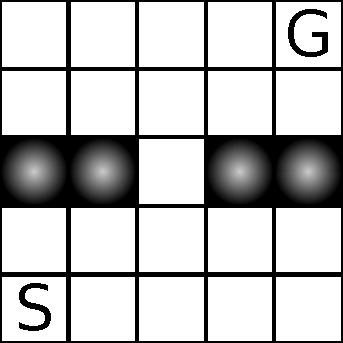
\includegraphics[scale=.55]{./imgs/gridHole/gridhole.pdf}
\caption{Structure of the grid world with holes problem.}
  \label{F:grid_hole_map}
\end{figure}
\begin{figure}[t]
\begin{minipage}{\columnwidth}
\centering
  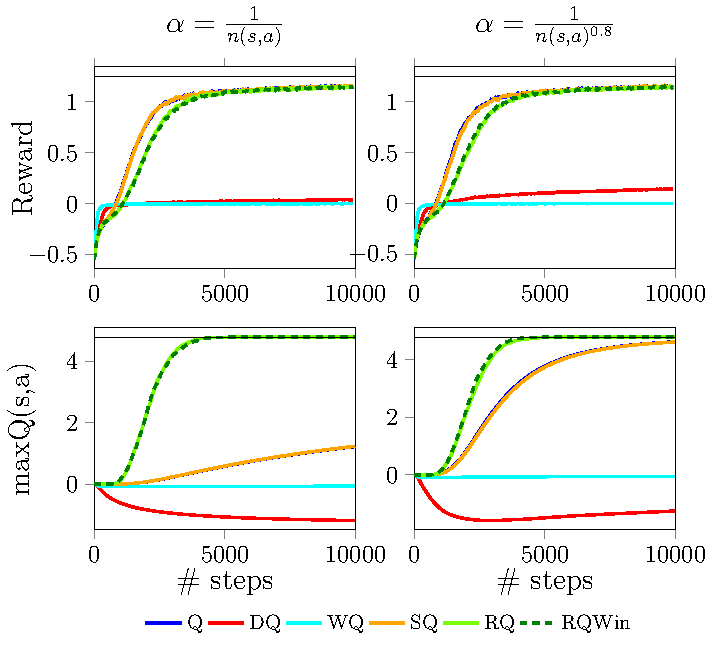
\includegraphics[scale=.7]{./imgs/gridHole/grid_hole.pdf}
\end{minipage}
  \caption{Mean reward per step (top) and maximum action-value estimate in the initial state (bottom) of all the other algorithms and of the best setting of \alg for this experiment. Results are averaged over $10000$ experiments.}
  \label{F:hole}
\end{figure}

This environment consists in a $5 \times 5$ grid with the initial position in the lower-left cell, there are $4$ actions and the transition model is deterministic, the goal position in the upper-right cell and four holes in the middle row in such a way that only the cell in the middle is walkable (Figure \ref{F:grid_hole_map}). The agent receives a reward of $0$ in all non-hole cells, a reward of $10$ when it reaches the goal state and a reward of $-10$ when it reaches a cell with a hole. The episode ends when the agent reaches a cell with a hole. The discount factor is $\gamma = 0.9$. \alg uses $\eta = 1$.
The learning rate settings are the same of the previous problem.

We consider this simple problem to highlight the limitations of pessimistic action-value estimates. In this MDP the optimal policy consists in avoiding the hole cells stepping through the state in the middle. Notice that in this state the episode terminates with negative reward with probability $\frac{\varepsilon}{2}$ due to the $\varepsilon$-greedy policy used for exploration, resulting in a very low value of the state especially at the beginning of learning. Figure \ref{F:hole} shows that while Q-Learning, Speedy Q-Learning and \alg behave similarly well, Double Q-Learning and Weighted Q-Learning obtain very poor results due to the pessimistic estimate of the value function of the state in the middle.

\subsection{On-policy learning}
As we have discussed in the previous sections, our approach can be used also in a on-policy setting. A simple on-policy version of our algorithm can be implemented by estimating the action-value function of the current policy in the same way of the SARSA algorithm, i.e. by using the action-value function of the next action. Let $u'$ be the next action sampled by the current policy in the current state, the on-policy update is:
\begin{align*}
\Rtilde_{t+1}(x,u) & \leftarrow\Rtilde_t(x,u)+\alpha_t(R(x,u,x')-\Rtilde_t(x,u)),\\
\Qtilde_{t+1}(x,u) & \leftarrow\Qtilde_t(x,u)+\beta_t(Q_t(x',u')-\Qtilde_t(x,u)).
\end{align*}

Figure \ref{F:sarsa} compares the windowed, on-policy version of \alg with the SARSA algorithm, in the Noisy Grid World environment. It is clear that our algorithm outperforms SARSA in this MDP.
Since this is an on-policy setting, at each step the algorithm is estimating the current policy action-value function, not the optimal one. Indeed, by looking at the mean reward per step, our approach estimates the current action-value function of the policy better than the SARSA algorithm, i.e. the estimated action-value function is coherent with the performance of the policy.

\begin{figure}[t]
\begin{minipage}{\columnwidth}
\centering
  \subfigure[$\alpha = \dfrac{1}{n(s,a)}$\label{F:sarsa_1}]{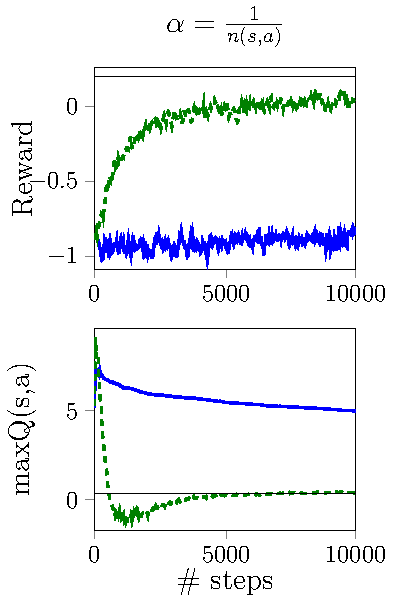
\includegraphics[scale=.7]{./imgs/sarsa/sarsa1.pdf}}\hspace{-.5cm}
  \subfigure[$\alpha = \dfrac{1}{n(s,a)^{0.8}}$\label{F:sarsa_08}]{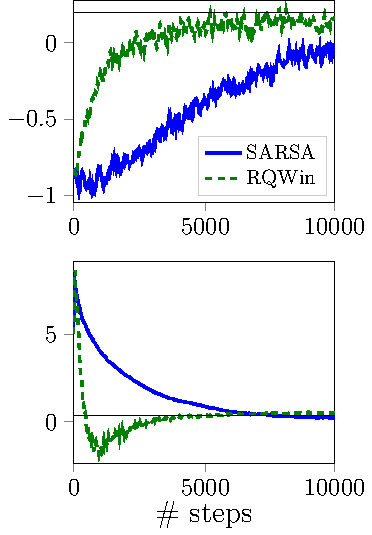
\includegraphics[scale=.7]{./imgs/sarsa/sarsa08.pdf}}
\end{minipage}
  \caption{Mean reward per step (top) and maximum action-value estimate in the initial state (bottom) of SARSA and of the on-policy windowed version of \alg for this experiment. Results are averaged over $1000$ experiments.}
  \label{F:sarsa}
\end{figure}

\section{Conclusion}
In this paper we proposed a method to improve the learning process in stochastic MDPs exploiting the structure of the Bellman operator. The decomposition in two components of the Bellman error allows to consider separately the sources of uncertainty. One of these components is the expected immediate reward whose uncertainty depends only on local properties of the MDP. The other component consists in the expected value function of the next state whose uncertainty depends on the policy (in an on-line setting), on the transition model and on other action-value estimates. We showed how the proposed method obtains good results in stochastic MDPs exploiting the information on the uncertainty of the estimates by adapting the learning rate according to it. Interestingly, this method is applicable both in off-policy and in on-policy settings; moreover, it is independent from the choice of the estimator of the expected value function of the next state.

In the experimental section, we empirically show that good results in highly stochastic MDPs can also be reached by algorithms that overestimates the action-value function. These results demonstrate that there seems not to be such a strong correlation between the underestimation of the action-value function and good performance in these kind of environments, as suggested in recent literature. Indeed, while the propagation of overestimates could lead to divergent estimates, in some cases this is not an issue as the optimal policy only depends on the order of the action-values. Moreover, our method is able to converge to the optimal action-value even with a initially high overestimation. It demonstrates how overestimation allows a better exploration given that the learning rate properly decreases. On the contrary, methods that underestimate the action-values suffer from poor exploration as we show in a simple deterministic environment.



% trigger a \newpage just before the given reference
% number - used to balance the columns on the last page
% adjust value as needed - may need to be readjusted if
% the document is modified later
%\IEEEtriggeratref{8}
% The "triggered" command can be changed if desired:
%\IEEEtriggercmd{\enlargethispage{-5in}}

% references section

% can use a bibliography generated by BibTeX as a .bbl file
% BibTeX documentation can be easily obtained at:
% http://mirror.ctan.org/biblio/bibtex/contrib/doc/
% The IEEEtran BibTeX style support page is at:
% http://www.michaelshell.org/tex/ieeetran/bibtex/
\bibliographystyle{IEEEtran}
% argument is your BibTeX string definitions and bibliography database(s)
\bibliography{biblio}

% that's all folks
\end{document}
